\documentclass[a4paper]{article}
\usepackage[slovene]{babel}
\usepackage[utf8]{inputenc}
\usepackage[T1]{fontenc}
\usepackage{graphicx}
\usepackage{bbm}
\usepackage{enumitem}
\usepackage{marvosym}
\usepackage{amssymb,amsmath}
\title{Upravljanje maloprodajnega prostora}
\author{Leon Horvat, Jernej Banevec \\ Finančni praktikum \\ Finančna matematika, Fakulteta za matematiko in fiziko}
\date{2018}



\begin{document}
\title{%
  Upravljanje omejenega maloprodajnega prostora za osnovne izdelke}

\author{Jernej Banevec, Leon Horvat}

\maketitle

\pagebreak

\section{Uvod}


Maloprodajne trgovine imajo veliko izbiro izdelkov, ki jih lahko vključijo v svojo ponudbo, hkrati pa so omejeni s prostorom v posamezni trgovini. Lahko se odločijo, da bodo imeli več različnih produktov z manjšimi zalogami na policah in posledično pogostejšim polnjenjem polic ali pa manj produktov z večjimi zalogami. Nepravilna izbira lahko vodi v nižji dobiček. Trgovci se morajo pri upravljanju maloprodajnega prostora odločiti, katere izdelke vključiti v svojo ponudbo ter optimizirati velikost zalog na policah in urnik njihovega polnjenja. Ti dve odločitvi sta tesno povezani, zato jih moramo obravnavati sočasno. 


Pri analizi problema se bova osredotočila na trgovine, ki imajo v svojo ponudbo vključene izdelke z dolgo življenjsko dobo in stabilnim povpraševanjem. 

Med trgovci sta se oblikovali dve strategiji za razporeditev izdelkov: strategija dodeljenega prostora in strategija skupnega prostora. Pri strategiji dodeljenega prostora ima vsak izdelek svoj točno določen prostor, pri strategiji skupnega prostora pa je dovoljeno deljenje prostora. Na primer trgovci lahko določenemu izdelku namenijo 20 centimetrov širine police, lahko pa neki skupini izdelkov namenijo prostor, v katerem je razporeditev odvisna od zaloge posameznega izdelka na polici; če ravno dopolnemo zalogo enega izdelka, mora biti ostalih manj, da je na polici dovolj prostora. Če je prostor dodeljen izdelku, je upravljanje urnika polnjenja polic manj zahtevno kot pri strategiji skupnega prostora. Pri slednji morajo biti trgovci na to bolj pozorni, ker lahko v primeru istočasnega polnjenja polic s temi izdelki zmanjka prostora. 

\vspace{4 mm}


Za zgled vzemimo 2 izdelka X in Y, ki imata oba enako velikost 1. Namenimo jima 10 enot prostora. Zalogi obeh se obnavljata na 6 dni. Če obnovimo obe zalogi hkrati, torej prvi dan, prostora na polici ni dovolj glede na povpraševanje izdelka. Če pa zalogo drugega obnovimo prvi dan, prvega pa četrti dan, potrebujemo manj prostora in 10 enot zadostuje povpraševanju obeh izdelkov. Opazimo, da pri uporabi strategije skupnega prostora porabimo manj prostora, vendar je potrebna koordinacija polnjenja zalog izdelkov, ki si delijo prostor.

\begin{figure}[ht]
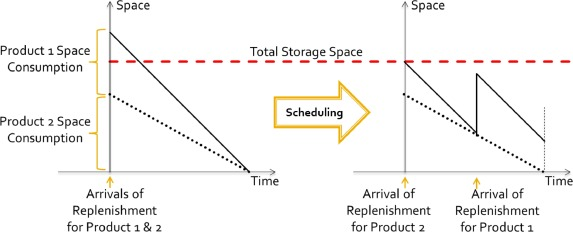
\includegraphics [scale = 0.8]{primerjava-strategij}
\caption{Poraba prostora strategij}
\end{figure}



\section{Modeliranje problema}

Upravljanje maloprodajnega prostora je formulirano kot nelinearen mešan celoštevilski program. Naj bo $\mathcal{P}= \{1, 2, ..., M\}$ indeksna množica možnih produktov. Predpostavimo, da imamo konstantno količino varnostne zaloge, ki je potrebna zaradi nihanja povpraševanja. Ta količina je lahko izračunana iz variacije povpraševanja in zahtevane ravni storitev, ki bo v našem primeru blizu 100 odstotkov, to pomeni da bo zelo majhna verjetnost, da katerega koli produkta zmanjka. Zaradi visoke zahtevane ravni storitev bomo v modelu upoštevali samo učinek substitucije izdelkov, ki jih nimamo v ponudbi, učinek substitucije razprodanih izdelkov pa zanemarimo. Predpostavimo tudi, da je povpraševanje eksogeno. Za vsak izdelek iz množice  $\mathcal{P}$, ki ni vključen v ponudbo, se del njegovega povpraševanja prenese na izdelke, ki so v ponudbo vključeni. Ta del povpraševanja zaradi substitucije manjkajočega izdelka je konstanten in neodvisen od ponudbe ostalih izdelkov. 

Pri problemu bomo predpostavili neodvisno polnjenje polic, torej da  ima vsak izdelek svoj strošek polnjenja. Lahko bi uporabili tudi strategijo kombiniranega polnjenja polic, pri kateri dodamo še strošek polnjenja izdelka iz določene skupine. Bolj natančno, če dopolnimo zalogo vsaj enega izdelka iz skupine, plačamo še ta dodaten strošek.

\vspace{3 mm}
Definirajmo:
\begin{itemize}
\item parametre:
\begin{itemize}
\item $ d_i $: prvotna stopnja povpraševanja po izdelku $i$,
\item $ w_{ij}$: delež povpraševanja izdelka $j$ prenesenega na izdelek $i$, če $j$-tega izdelka ni v ponudbi; $w_{ii} = 1$,
\item $ v_i $: dobiček pri $i$-tem izdelku,
\item $ h_i $: strošek hranjenja izdelka $i$ na polici,
\item $ k_i $: cena polnjenja izdelka $i$, 
\item $ \theta_i $: koeficient količine varnostne zaloge izdelka $i$,
\item $ C $: ves prostor, ki je na voljo v trgovini,
\item $ c_i $: prostor, ki ga zasede izdelek $i$.
\end{itemize}

\item odločitvene spremenljivke:
\begin{itemize}
\item $ y_i $: indikator, ki nam pove, ali je izdelek $i$ vključen v ponudbo,
\item $ Q_i $: število naročenih izdelkov $i$.
\item $ T $: čas cikla dopolnjevanja zalog na policah,
\item $ \tau_i $: čas poljnjenja izdelka $i$ v ciklu,
\item $ t_{ij}$: čas med polnjenjem izdelka $i$ in $j$.
\end{itemize}

\item pomožne spremenljivke:
\begin{itemize}
\item $ x_{ij} $: indikator substitucije iz izdelka $j$ na izdelek $i$; $x_{ij} = y_i (1-y_j)$, če $j \ne i$ in $x_{ij} = y_i$, če  $j = i$,
\item $ s_i $: končna efektivna stopnja povpraševanja po $i$-tem izdelku; $s_i = y_i (d_i + \sum_{j \ne i} w_{ij} d_j (1-y_j)) = \sum_j  w_{ij} d_j x_{ij}.$
\end{itemize} 
\end{itemize}

Med parametri in spremenljivkami morajo veljati naslednje zveze:
\begin{enumerate}[label={[\arabic*]}]
\item $ s_i = \sum_j w_{ij} d_j x_{ij}, \forall i$,
\item $ x_{ij} \leq y_i, \forall i, j  $,
\item $ x_{ij} \leq 1 - y_j, \forall i \ne j$,
\item $ y_i \in \{0,1\}$,
\item $ x_{ij} \geq 0, \forall i,j$,
\item $Q_i = s_iT$,
\item $t_{ij} = (\tau_j - \tau_i) * \mathbbm{1}\{\tau_i \leq \tau_j\} +  (T + \tau_j - \tau_i) * \mathbbm{1}\{\tau_i > \tau_j\} $, če $i < j$ in $ (\tau_j - \tau_i) * \mathbbm{1}\{\tau_i < \tau_j\} +  (T + \tau_j - \tau_i) * \mathbbm{1}\{\tau_i \geq \tau_j\} $, če $i \geq j $,
\item $t_{ij} \geq 0, t_{ii} = T$,
\item $t_{ij} + t_{ji} = T, \forall i \ne j $,
\item $t_{ij} - t_{ik} = z_{kj} t_{kj} - z_{jk} t_{jk} \forall i \ne j \ne k$,
\item $z_{kj} + z_{jk} = 1, \forall j \ne k$,
\item $z_{ij} \in \{ 0, 1\}, \forall i, j$,
\item $\sum_j c_j s_j (t_{ij} + T \theta_j) \leq C, \forall i$.


\end{enumerate}

Prvi pogoj definira končno efektivno stopnjo povpraševanja, drugi in tretji pogoj definirata $x$ s pomočjo $y$. Pogoji $[4]$, $[5]$ in $[8]$ določajo definicijsko območje $y$, $x$ in $t$. Pogoj $[6]$ nam zagotavlja, da je povpraševanje v ciklu $s_i T$ enako količini naročenih izdelkov $Q_i$ za dopolnitev zalog. Pogoj $[7]$ predstavlja zvezo med $\tau$ in $t$. Iz definicije $t$ dobimo pogoj $[9]$. $[10]$, $[11]$ in $[12]$ predstavljajo trikotniško relacijo med $t$-ji.  Pogoj $[13]$ nam zagotavlja, da je ob vsakem času polnjenja polic dovolj prostora za vse izdelke. 




Naš cilj je maksimizacija dobička, pri zgornjih omejitvah. Maksimizacijska funkcija:

$$  \max  \sum_{i \in \mathcal{P}} ( v_i s_ i - H_i  Q_i - \frac{k_i y_i}{T})   $$ 

\vspace*{1 mm}
Maksimiziramo torej neto dobiček (celoten dobiček zmanjšan za stroške hranjenja izdelka na polici in polnjenja izdelka). To je mešani celoštevilski program z nelinearno optimizacijsko funkcijo. Ker je ta problem težko rešljiv, obstajajo metode, ki zmanjšajo kompleksnost reševanja. Te metode bova predstavila posebej za vsako strategijo polnjenja polic.

\pagebreak
\section{Strategija skupnega prostora}

Opazimo, da sta v prej navedenem optimizacijskem problemu vkoreninjena dva podproblema. Prvi problem odloča o tem, katere izdelke bomo vključili v ponudbo, drugi pa se ukvarja z urnikom polnjenja polic. 
Problem izbire ponujenih izdelkov:
$$g(T, t) = max_{s, x, y}  v' s - T \cdot H' s - \frac{1}{T} \cdot k' y $$
p.p.

$[1] - [5]$ in $[13]$

\vspace*{3 mm}

Ta problem je relativno lahko prevesti na linearen program. Drugi problem je bolj zapleten. 
Problem urnika dopolnjevanja zalog:
$$f(s, y) = max_{T, t, z}  v' s - T \cdot H' s - \frac{1}{T} \cdot k' y $$
p.p.

$[8] - [13]$

\vspace*{3 mm}

Z nekaj zvitimi prijemi ta problem poenostavimo: Definiramo $B$, ki predstavlja velikost prostora pri dani izbiri izdelkov v ponudbi in urniku polnjenja zalog, ter $\beta$, ki je enaka $\frac{B}{T}$ in glede na podani $s$ dobimo formuli za izračun optimalnega $T$: 
$T^{*} (s) = min\{\sqrt{\frac{k' y}{H' s}}, \frac{C}{\beta(s)}  \}$, kjer optimalni $\beta^*  (s) = \sum_{i \in \mathcal{P}} (s_i c_i \cdot \sum_{j = 1}^{i} s_j c_j) \sum_{i \in \mathcal{P}} s_i c_i $.

\vspace*{1 mm}
Če imamo vrednosti, pri katerih prvotni optimizacijski problem doseže maksimalno vrednost $v ^ *$, potem to vrednost dosežeta tudi oba podproblema. Če obnovimo, smo začetni optimizacijski problem razdelili na dva podproblema, kjer rešitev enega predstavlja vhodni podatek za drugega. To je tudi ideja za algoritem strategije skupnega prostora.

\begin{enumerate}
\item $k = 0, s^k = d, t^k = 0, T^k = 0$ in postavimo zaustavitveni kriterij $L$, ki predstavlja spodnjo mejo, maksimalno število korakov $S$, ter $\epsilon > 0$.
\item $k = k+1$ in rešimo $f(s ^{k-1})$ in dobimo $T^k$ in $t^k$ .
\item Rešimo $g(T^k, t^k)$ in dobimo $s^k$.
\item Če je $L  + \epsilon> f(s^k)$ ali  presežemo maksimalno število korakov ($k > S$), potem končamo.
\item $L = f(s^k)$ in se vrnemo na prvi korak.
\end{enumerate}

\pagebreak
\section{Strategija dodeljenega prostora}

Če je prostor dodeljen vsakemu produktu, je dopolnjevanje zalog enostavnejše in ne potrebujemo usklajevati urnika polnjenja zalog in skupnega časa cikla dopolnjevanja zalog na policah. Torej vsak produkt ima svoj cikel. Namesto pogoja $[13]$ definiramo drugačen pogoj, ki nam zagotavlja prostor na policah: $[14]\hspace*{1 mm} \sum_{i \in \mathcal{P}} (1 + \theta_i) c_i s_i T_i \leq C$. Sledi, da je problem pri strategiji dodeljenega prostora naslednji:
$$ \max  \sum_{i \in \mathcal{P}} ( v_i s_ i - H_i  s_i T_i - \frac{k_i y_i}{T_i})  $$
p.p.

$[1] - [5]$ in $[14]$

\vspace*{1 mm}
Ker je $T$ vsebovan samo v pogoju $[14]$, lahko z metodo Lagrangejevih multiplikatorjev pridemo do sledeče formule:
$T^*_i(s, \lambda) = \sqrt{\frac{k_i y_i}{s_i ((1+\theta_i)c_i\lambda + H_i}}$

Ideja algoritma strategije dodeljenega prostora:
\begin{enumerate}
\item $k = 0, s^k = d$
\item $k = k + 1$, s pomočjo prej podane formule  za optimalen $T$ izračunamo najmanjšo $\lambda \geq 0$, tako da bo za dane parametre še zadoščeno pogoju $[14]$.
\item Za dano $\lambda$ izračunamo optimalen $T^k$.
\item Rešimo DSS s podanim $T^k$ da dobimo $s^k$; če $s$ konvergira, potem je $s^k$ rešitev, drugače gremo na korak $2$.
\end{enumerate}

<<<<<<< HEAD
([2252.311818408007, 3143.1831609044366, 4280.116962968127, 5541.585444746526, 6501.973186455406, 7530.25347214121, 8754.290465617662, 9786.694783226574, 10856.17098199368], [2345.602636111844, 3207.5533302456315, 4256.5370910694555, 5199.690682474628, 5812.365118850423, 6896.47033920601, 7296.699005079152, 7921.030172898909, 8550.78511195774])

([4479.623745426181, 4400.655447289399, 4220.196508734808, 4450.160053869553, 4497.607949806566, 4074.4941779577302, 4141.5765760799295, 4410.311184662159, 4408.3146147519155, 4358.7662140877665, 4270.6329077838], [3269.550976759267, 3767.877518091663, 3833.1889714146832, 4271.391783013575, 4524.03584973299, 4211.05110540659, 4272.952835126323, 4606.627202979208, 4598.773459930919, 4553.839625801792, 4478.4311296320975])
=======
\section{Generiranje podatkov}


Vzela sva širok nabor parametrov, ki so večinoma povzeti po viru. Vsak parameter je odvisen od $U$, ki predstavlja naključno generirano število na odprtem intervalu $(0,1)$. $M$ je število produktov, ki lahko nastopajo v ponudbi trgovin. Analizo sva delala z najmanj dvema in največ desetimi produkti. Pri vsakem produktu sva za vsako lastnost generirala novo število $U$.

 \vspace*{3 mm}

\begin{tabular}{ l l | l l }
	\hline
  $C$ & $(5 + 30 U) \cdot M$ & $ \Delta_v $ & $8 U$\\
  $CV_i$ & $U \cdot CV_B$ & $k_i$ & $\bar{k} + (U - 0.5) \Delta_k$\\
  $CV_B$ & $1 + 9 U$ & $ \bar{k}$ & $0.03 + 0.07 U$\\
  $\theta_i$ & $ 1.65 \cdot CV_i$ & $ \Delta_k$ & $0.05 U$\\
  $d_i$ & $\bar{d} + (U - 0.5) \Delta_d$ & $ c_i$ & $\bar{c} + (U - 0.5) \Delta_c$\\
  $\bar{d}$ & $50 + 100 U$ & $\bar{c}$ & $ 0.05 + 0.1 U$\\
  $\Delta_d$ & $80 U$ & $\Delta_c$ & $0.09 U$\\
  $ v_i$ & $\bar{v} + (U - 0.5) \Delta_v$ & $H_i$ & $ c_i \cdot (\frac{1}{2} + \theta_i)$\\
  $ \bar{v}$ & $ 5 + 10 U$ & &\\
	\hline
\end{tabular}


\section{Analiza}






\section{Vir}

\begin{enumerate}
\item Zhang W. , Rajaram K. 2017. Managing limited retail space for basic products: Space sharing vs. space dedication. \textit{European Journal of Operational Research}. 263, 768 - 781
\end{enumerate}
>>>>>>> c3ea4d1c834e7e7e64a6c64eee7e22484fdf10ec

\end{document}